\chapter{NIXSW of QA on the Ag(100) surface}

The following sections show the \ac{NIXSW} spectra and the resulting fit parameters for the C1s, O1s and N1s core levels of \ac{QA} on the Ag(100) surface in the $\alpha$- and $\beta$-phase. For each core level, one section is dedicated to the $\alpha$-phase and one section to the $\beta$-phase, respectively.

To obtain the \ac{NIXSW} spectra, a series of 31 \ac{XPS} measurements at different photon energies around the (200) Bragg reflection of the Ag(100) surface were performed. Each \ac{XPS} spectrum was fitted with the same model as used for the static \ac{XPS} spectra in \autoref{chap:XPS}, where the \ac{FWHM} and \ac{BE} of the individual peaks were fixed and only the peak area was varied. The resulting normalized photoelectron yield of the individual peaks were then plotted against the photon energy to obtain the \ac{NIXSW} spectra.

\section{The \texorpdfstring{$\alpha$}{alpha}-phase}
\label{chap:NIXSW-alpha}

In the following sections, the \ac{NIXSW} spectra for the $\alpha$-phase of \ac{QA} on the Ag(100) surface are presented. They are divided into C1s, N1s, and O1s core levels.

\subsection{C1s NIXSW spectra}
\label{chap:C1s-NIXSW}

The C1s \ac{NIXSW} spectra of \ac{QA} on the Ag(100) surface in the $\alpha$-phase are shown in \autoref{fig:NIXSW-C1s-alpha}.

At the bottom of \autoref{fig:NIXSW-C1s-alpha}, the measured reflectivity curve of the Ag(100) surface around the (200) Bragg reflection is shown. The different data points and the fitted curve of the C1s \ac{NIXSW} spectra are shown for the different \ac{XPS} components from \autoref{tab:XPS-C1s-fit} in different colors. At the top of the figure, the sum of all C1s components is shown. For a better visibility, the different \ac{NIXSW} spectra are shifted vertically by 1.

\begin{figure}[H]
    \centering
    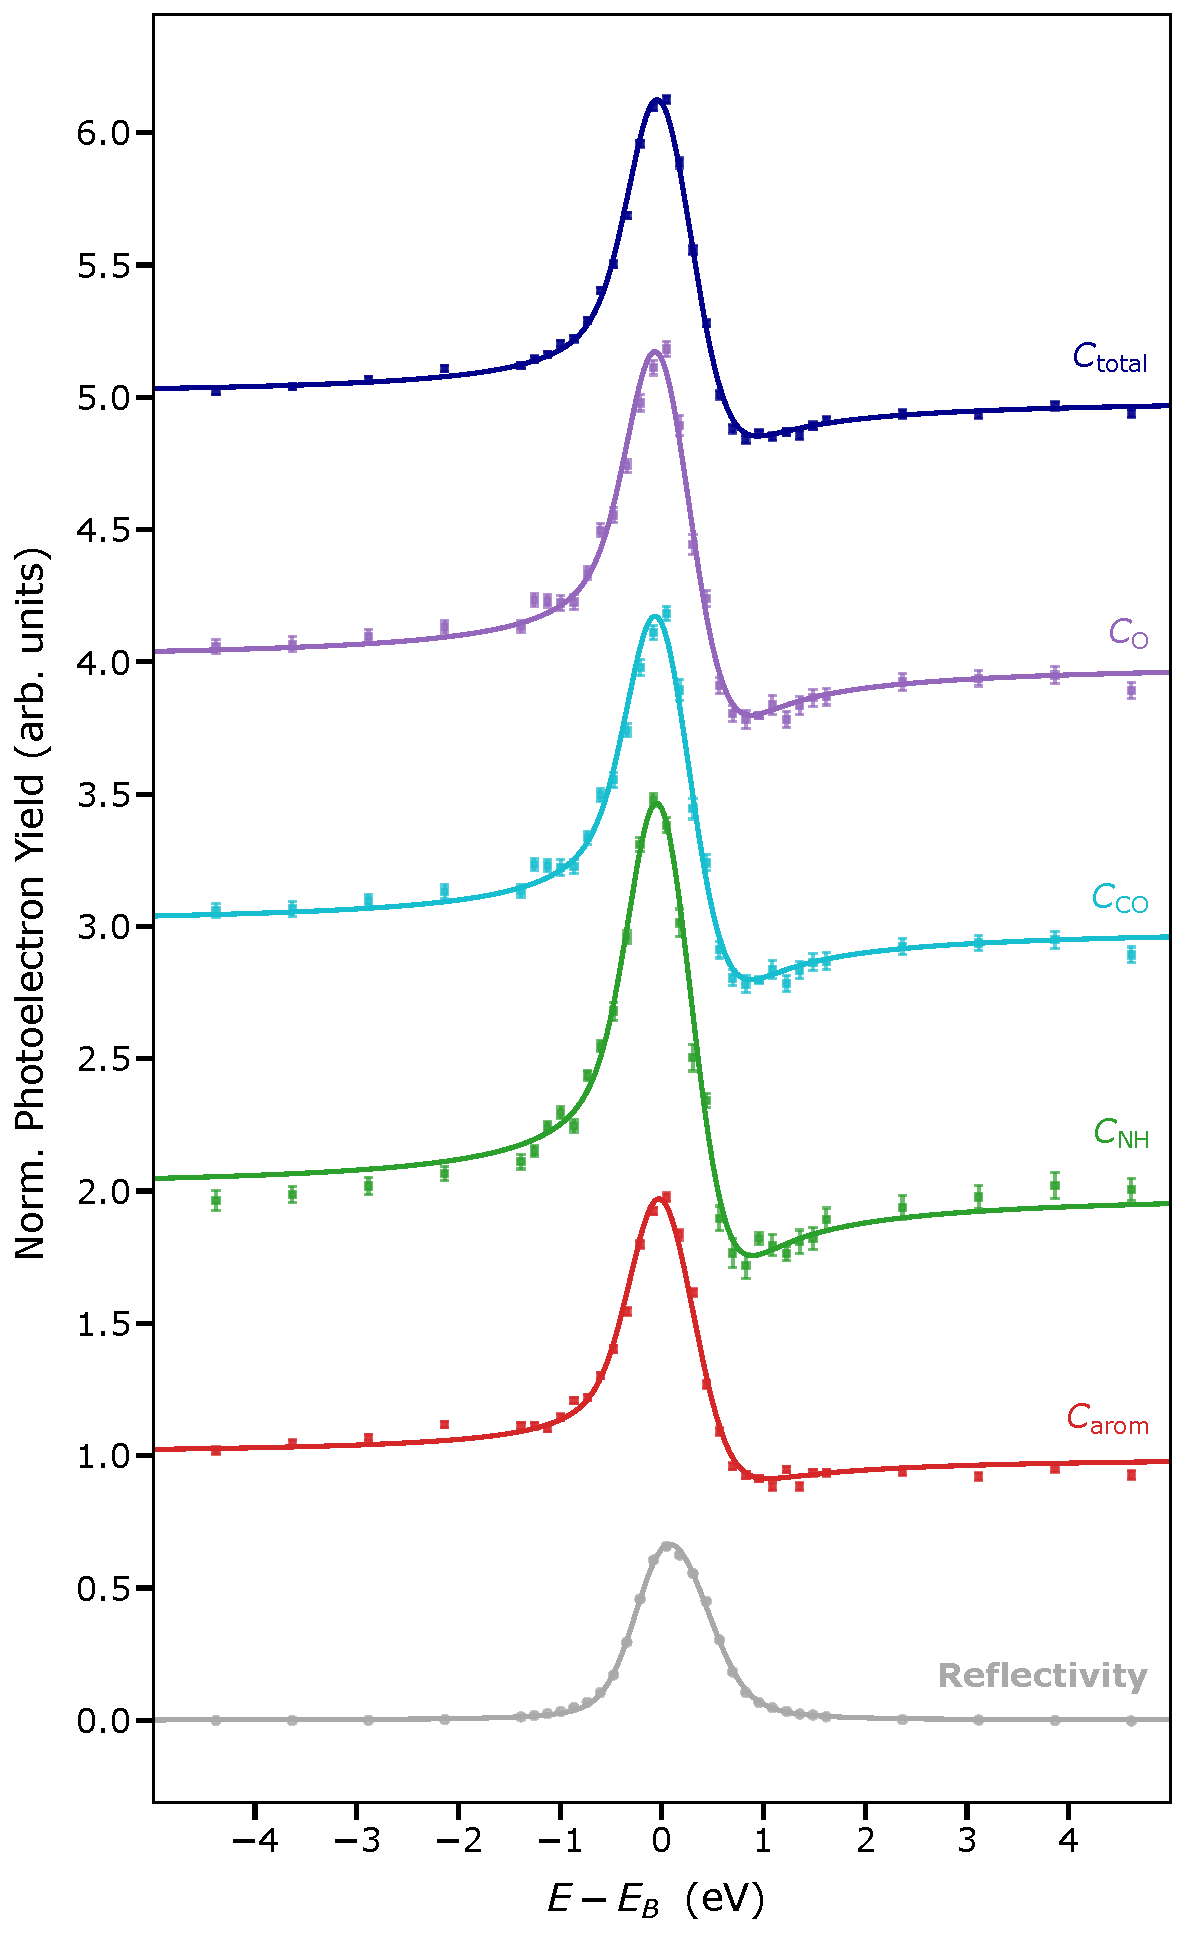
\includegraphics[width=0.8\textwidth]{images/NIXSW/NIXSW_C1s_Alpha.pdf}
    \caption{C1s \ac{NIXSW} spectra of \ac{QA} on the Ag(100) surface in the $\alpha$-phase. The sum of all components is shown at the top, followed by the individual components $\mathrm{C_{arom}}$, $\mathrm{C_{NH}}$, $\mathrm{C_{CO}}$ and $\mathrm{C_{O}}$ and the reflectivity at the bottom. For a better visibility, the different \ac{NIXSW} spectra are shifted vertically by 1. The fit parameter from \autoref{tab:XPS-C1s-fit} were used for the individual \ac{XPS} spectra.}
    \label{fig:NIXSW-C1s-alpha}
\end{figure}

\autoref{fig:NIXSW-C1s-alpha} shows that the different C1s components have distinct \ac{NIXSW} spectra. Consequently, the different C atoms in the \ac{QA} molecule on the Ag(100) surface have distinct coherent fractions and positions. The resulting fit parameters for the different C1s components are summarized in \autoref{tab:NIXSW-C1s-alpha}.

\begin{table}[H]
	\centering
	\caption{Resulting coherent positions $p_\mathrm{c}$ and coherent fractions $p_\mathrm{c}$ for the different C1s components of \ac{QA} on the Ag(100) surface in the $\alpha$-phase from \autoref{fig:NIXSW-C1s-alpha}. The distance $z_{200}$ is calculated from the coherent position $p_\mathrm{c}$.}
	\begin{tabular}{@{}cccc@{}} \toprule
		 & $p_\mathrm{c}$ & $f_\mathrm{c}$ & $z_{200}$ (\si{\angstrom}) \\
		\midrule
		$\mathrm{C_{arom}}$ & $0.459 \pm 0.007$ & $0.369 \pm 0.015$ & $2.981 \pm 0.014$ \\
		$\mathrm{C_{NH}}$ & $0.438 \pm 0.006$ & $0.811 \pm 0.031$ & $2.938 \pm 0.012$ \\
		$\mathrm{C_{CO}}$ & $0.469 \pm 0.007$ & $0.615 \pm 0.020$ & $3.001 \pm 0.014$ \\ 
		$\mathrm{C_{O}}$ & $0.458 \pm 0.011$ & $0.436 \pm 0.029$ & $2.979 \pm 0.022$ \\
        $\mathrm{C_{total}}$ & $0.455 \pm 0.004$ & $0.523 \pm 0.012$ & $2.973 \pm 0.008$ \\
		\bottomrule
	\end{tabular}
	\label{tab:NIXSW-C1s-alpha}
\end{table}



\autoref{tab:NIXSW-C1s-alpha} shows that the coherent fractions $f_\mathrm{c}$ vary between 0.369 and 0.811, with a coherent fraction $f_\mathrm{c}$ of 0.523 for the total C1s signal. The $\mathrm{C_{NH}}$ peak has the highest coherent fraction $f_\mathrm{c}$ of 0.811, followed by the $\mathrm{C_{CO}}$ peak with a coherent fraction $f_\mathrm{c}$ of 0.615. The $\mathrm{C_{arom}}$ and $\mathrm{C_{O}}$ peaks have lower coherent fractions $f_\mathrm{c}$ of 0.369 and 0.436, respectively. The two peak with the highest coherent fractions $f_\mathrm{c}$ correspond to the C atoms that are not bond to hydrogen atoms and are part of two 6 membered rings in the \ac{QA} molecule.

Furthermore, the different C1s components have coherent positions $p_\mathrm{c}$ between 0.438 and 0.469, which results in a coherent position $p_\mathrm{c}$ of 0.455 for the total C1s signal. These values correspond to distances $z_{200}$ between 2.938~\si{\angstrom} and 3.001~\si{\angstrom}, with a distance of 2.973~\si{\angstrom} for the total C1s signal. 

In total, there is only a deviation of 0.063~\si{\angstrom} in the distance $z_{200}$. Taking the errors of the distance $z_{200}$ into account, the deviations of the adsorption height may be even smaller. This indicates that all C atoms in the \ac{QA} molecule on the Ag(100) surface in the $\alpha$-phase are located at similar heights above the surface, with only small differences between the different C atoms. 

However, the averaged distance of the C atoms to the Ag(100) surface of around 2.973~\si{\angstrom} is lower than the sum of the van der Waals radii for C/Ag, which is 3.42~\si{\angstrom}.\autocite{Bondi1964} In comparison, the binding distance of the C atoms in the $\alpha$-phase are 13~\% closer to the surface than the van der Waals radii. The binding distance of the C atoms in the $\alpha$-phase is also comparable to other $\pi$-conjugated molecules on the Ag(100) surface, such as \ac{PTCDA} with a binding distance of 2.84~\si{\angstrom}.\autocite{Bauer2014} Additionally, the binding distance of pentacene on Ag(111), which is between 2.99~\si{\angstrom} and 3.13~\si{\angstrom},\autocite{Burker2014} is a little higher than the binding distance of the C atoms in the $\alpha$-phase. The differences between \ac{QA} and pentacene are the functional groups in \ac{QA}, namely the amine and carbonyl groups, which can interact with the Ag(100) surface and thus lead to a stronger interaction between the C atoms and the Ag(100) surface in \ac{QA} compared to pentacene, which does not have any functional groups.

\newpage 
\subsection{N1s NIXSW spectra}

In the following, the N1s \ac{NIXSW} spectra of \ac{QA} on the Ag(100) surface in the $\alpha$-phase are presented in \autoref{fig:NIXSW-N1s-alpha}. At the bottom of the figure, the measured reflectivity curve of the (200) Bragg reflection is shown. The data points and the fitted curve of the N1s \ac{NIXSW} spectrum for the $\mathrm{N1}$ component are shown above the reflectivity. For a better visibility, the different curves are shifted vertically by 1.

\begin{figure}[htbp]
    \centering
    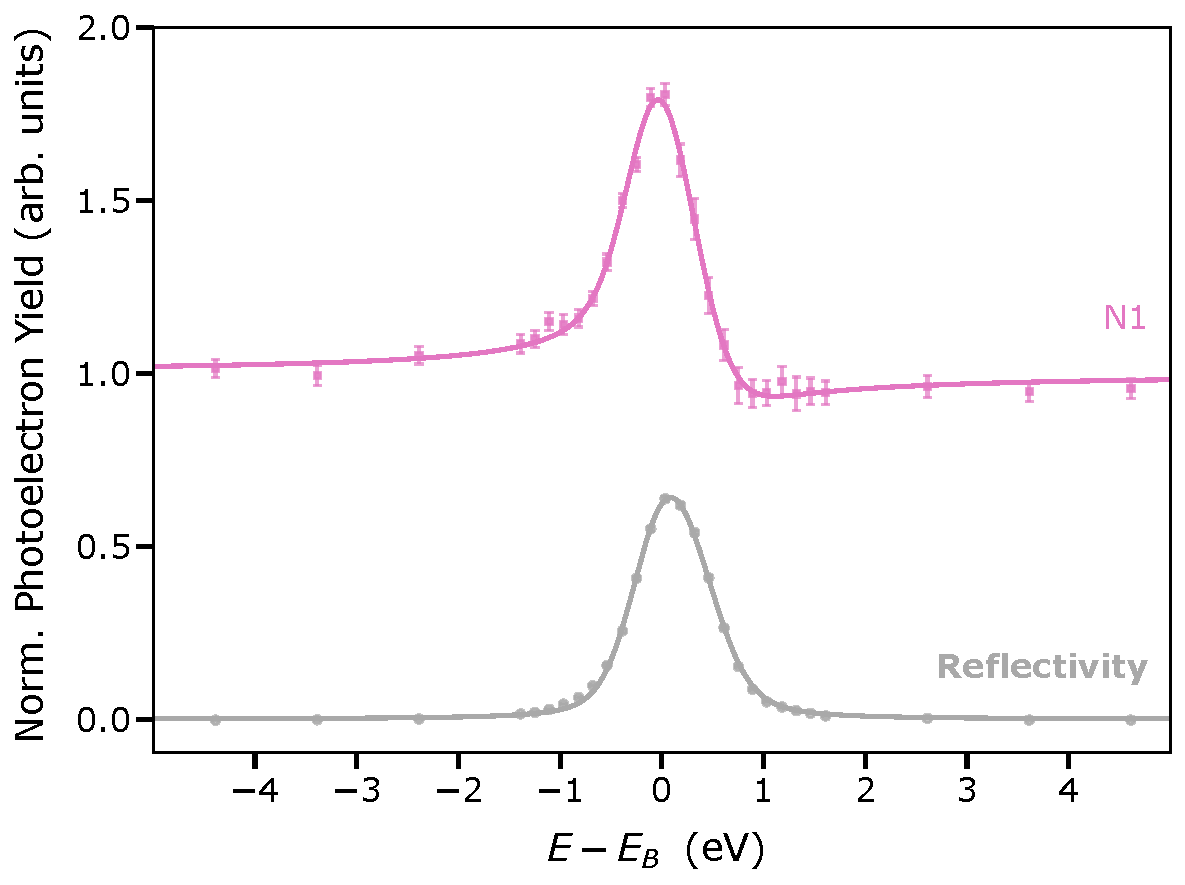
\includegraphics[width=0.8\textwidth]{images/NIXSW/NIXSW_N1s_Alpha.pdf}
    \caption{N1s \ac{NIXSW} spectra of \ac{QA} on the Ag(100) surface in the $\alpha$-phase. The component $\mathrm{N1}$ is shown at the top and the reflectivity at the bottom. For a better visibility, the different \ac{NIXSW} spectra are shifted vertically by 1. The fit parameter from \autoref{tab:XPS-N1s-fit} were used for the individual \ac{XPS} spectra.}
    \label{fig:NIXSW-N1s-alpha}
\end{figure}

\autoref{fig:NIXSW-N1s-alpha} shows that the N1s \ac{NIXSW} spectrum of the $\mathrm{N1}$ component exhibits a similar peak as the C1s \ac{NIXSW} spectra. The resulting fit parameters and the distance $z_{200}$ for the N1s component are summarized in \autoref{tab:NIXSW-N1s-alpha}.

\begin{table}[htbp]
	\centering
	\caption{Resulting coherent positions $p_\mathrm{c}$ and coherent fractions $p_\mathrm{c}$ for the different N1s components of \ac{QA} on the Ag(100) surface in the $\alpha$-phase from \autoref{fig:NIXSW-N1s-alpha}. The distance $z_{200}$ is calculated from the coherent position $p_\mathrm{c}$.}
	\begin{tabular}{@{}cccc@{}} \toprule
		 & $p_\mathrm{c}$ & $f_\mathrm{c}$ & $z_{200}$ (\si{\angstrom}) \\
		\midrule
		$\mathrm{N1}$ & $0.499 \pm 0.009$ & $0.288 \pm 0.013$ & $3.062 \pm 0.018$ \\
		\bottomrule
	\end{tabular}
	\label{tab:NIXSW-N1s-alpha}
\end{table}

\autoref{tab:NIXSW-N1s-alpha} shows that the N1s component has a coherent position $p_\mathrm{c}$ of 0.499, which corresponds to a distance $z_{200}$ of 3.062~\si{\angstrom}. This distance is higher than the distance of the C atoms to the Ag(100) surface of 2.973~\si{\angstrom}, showing that the N atoms are located farther away from the Ag(100) surface than the C atoms in the \ac{QA} molecule on the Ag(100) surface in the $\alpha$-phase. The sum of the van der Waals radii for N/Ag, which is 3.30~\si{\angstrom}\autocite{Bondi1964}, is larger than the binding distance of the N atoms, however, the binding distance of the N atoms in the $\alpha$-phase is only 7~\% closer to the surface than the van der Waals radii.

The coherent fraction of the N1 component $f_\mathrm{c}$ is 0.288. This coherent fraction is significantly lower than the coherent fractions of the C1s components, which are between 0.369 and 0.811. Compared to the merocyanine HB238 on the Ag(100) surface, which has a coherent fraction of 0.234 for the N1s component,\autocite{Kny2025} the N atoms in the \ac{QA} molecule on the Ag(100) surface in the $\alpha$-phase have a higher degree of order. However, there are also organic molecules like azobenzen on the Ag(111) surface, that exhibit coherent fractions of almost 0.5\autocite{Mercurio2014}, which is significantly higher than the coherent fraction of the N atoms in the \ac{QA} molecule on the Ag(100) surface in the $\alpha$-phase.

\newpage
\subsection{O1s NIXSW spectra}

In the following, the O1s \ac{NIXSW} spectra of \ac{QA} on the Ag(100) surface in the $\alpha$-phase are presented in \autoref{fig:NIXSW-O1s-alpha}. Again, the reflectivity curve of the (200) Bragg reflection is shown at the bottom and the data points and fitted curve of the O1s \ac{NIXSW} spectrum for the $\mathrm{O1}$ component at the top. For a better visibility, the different curves are shifted vertically by 1.

\begin{figure}[htbp]
    \centering
    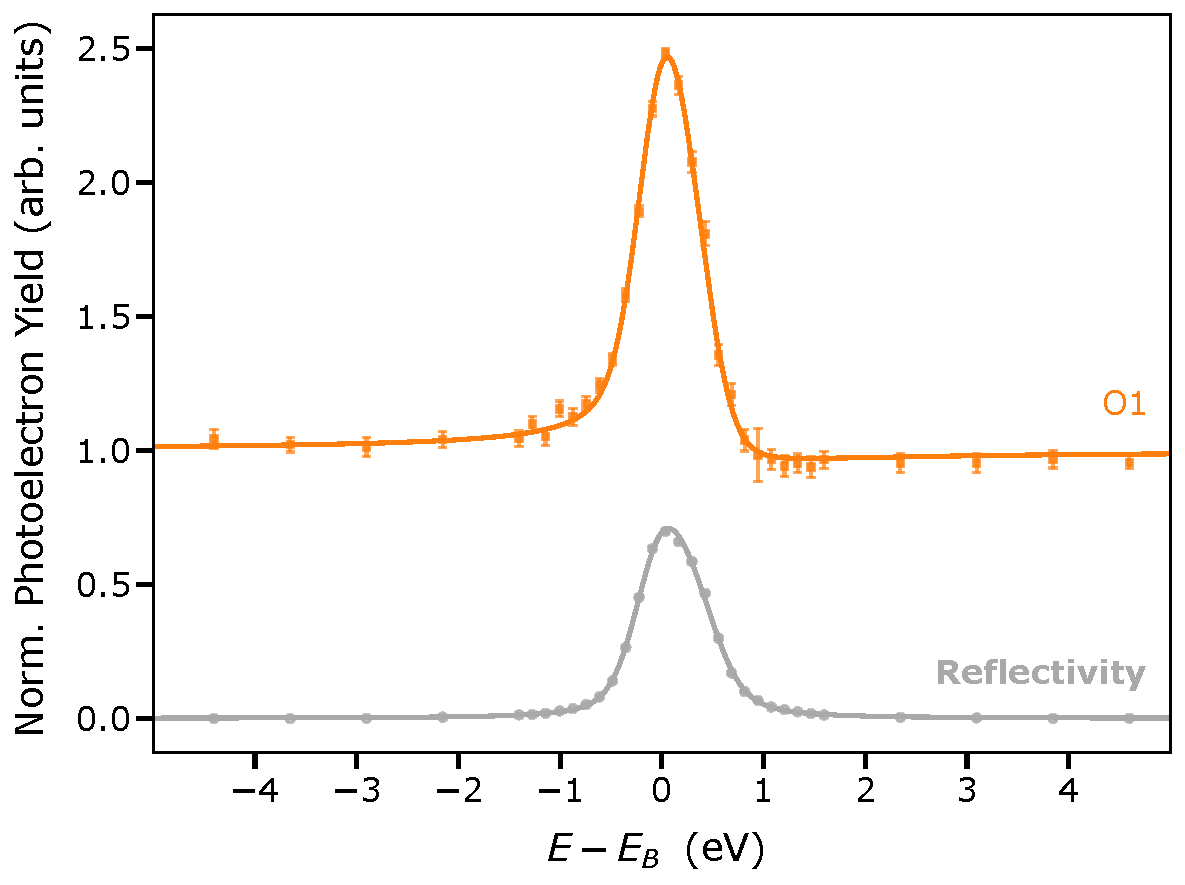
\includegraphics[width=0.8\textwidth]{images/NIXSW/NIXSW_O1s_Alpha.pdf}
    \caption{O1s \ac{NIXSW} spectra of \ac{QA} on the Ag(100) surface in the $\alpha$-phase. The component $\mathrm{O1}$ is shown at the top and the reflectivity at the bottom. For a better visibility, the different \ac{NIXSW} spectra are shifted vertically by 1. The fit parameter from \autoref{tab:XPS-O1s-fit} were used for the individual \ac{XPS} spectra.}
    \label{fig:NIXSW-O1s-alpha}
\end{figure}

The O1s \ac{NIXSW} spectrum of the $\mathrm{O1}$ component in \autoref{fig:NIXSW-O1s-alpha} also shows a similar behaviour as the C1s and N1s \ac{NIXSW} spectra. The resulting fit parameters for the O1s component are summarized in \autoref{tab:NIXSW-O1s-alpha}.

\begin{table}[htbp]
	\centering
	\caption{Resulting coherent positions $p_\mathrm{c}$ and coherent fractions $p_\mathrm{c}$ for the different O1s components of \ac{QA} on the Ag(100) surface in the $\alpha$-phase from \autoref{fig:NIXSW-O1s-alpha}. The distance $z_{200}$ is calculated from the coherent position $p_\mathrm{c}$.}
	\begin{tabular}{@{}cccc@{}} \toprule
		 & $p_\mathrm{c}$ & $f_\mathrm{c}$ & $z_{200}$ (\si{\angstrom}) \\
		\midrule
		$\mathrm{O1}$ & $0.332 \pm 0.004$ & $0.546 \pm 0.016$ & $2.721 \pm 0.008$ \\
		\bottomrule
	\end{tabular}
	\label{tab:NIXSW-O1s-alpha}
\end{table}

\autoref{tab:NIXSW-O1s-alpha} shows that the O1 component has a coherent position $p_\mathrm{c}$ of 0.332, which corresponds to a distance $z_{200}$ of 2.721~\si{\angstrom}. In comparison to the C and N atoms, the O atoms are located closer to the Ag(100) surface in the $\alpha$-phase. The sum of the van der Waals radii for O/Ag, which is 3.24~\si{\angstrom}\autocite{Bondi1964}, is 16~\% larger than the binding distance of the O atoms. This is a significant difference compared to the C and N atoms, which are only 13~\% and 7~\% closer to the surface than the van der Waals radii, respectively. 

In comparison to \ac{PTCDA} with a coherent position $p_\mathrm{c}$ of 0.24, resulting in a adsorption height of 2.53~\si{\angstrom}\autocite{Bauer2014} the O atoms in the \ac{QA} molecule on the Ag(100) surface in the $\alpha$-phase are located farther away from the surface. This is the same results as for the C atoms in \ac{QA} and \ac{PTCDA}, which also show a higher binding distance for \ac{QA} compared to \ac{PTCDA}.

The coherent fraction of the O1 component $f_\mathrm{c}$ is 0.546, which is significantly higher than the coherent fraction of the N1 component of 0.288. Furthermore, the coherent fraction of the O1 component is also higher than the coherent fractions of the $\mathrm{C_{arom}}$ and $\mathrm{C_{O}}$ components, which are 0.369 and 0.436, respectively. However, the coherent fraction of the O1 component is lower than the coherent fractions of the $\mathrm{C_{NH}}$ and $\mathrm{C_{CO}}$ components, which are 0.811 and 0.615. This shows that the degree of order for the O1 component is located in between the different C1s components and the N1s component, resulting in a medium degree of order for the O atoms in the \ac{QA} molecule on the Ag(100) surface in the $\alpha$-phase.
 

\newpage
\subsection{Discussion of the \texorpdfstring{$\alpha$}{alpha}-phase}

In the following, the coherent positions $p_\mathrm{c}$ and coherent fractions $f_\mathrm{c}$ for the different core levels of \ac{QA} on the Ag(100) surface in the $\alpha$-phase will be discussed in detail and compared to each other.

As an overview of the resulting coherent positions and fractions for the different core levels of \ac{QA} on the Ag(100) surface in the $\alpha$-phase, an Argand representation is shown in \autoref{fig:Argand-alpha}. Here, the coherent position $p_\mathrm{c}$ is represented as the angle and the coherent fraction $f_\mathrm{c}$ as the distance from the origin.

\begin{figure}[htbp]
	\centering
	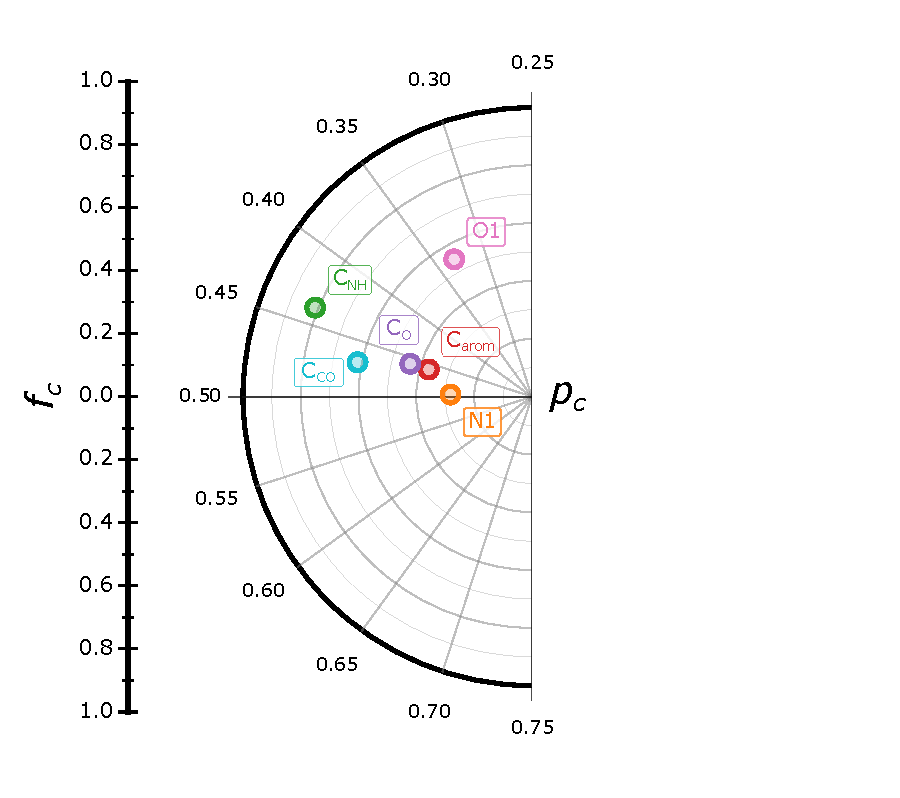
\includegraphics[width=0.7\textwidth]{images/NIXSW/Argand_Alpha_2.pdf}
	\caption{Argand representation for \ac{QA} on the Ag(100) surface in the $\alpha$-phase for the C1s, N1s, and O1s core levels.}
	\label{fig:Argand-alpha}
\end{figure}

As the coherent positions $p_\mathrm{c}$ are directly proportional to the adsorption heights, the following discussion of the coherent positions $p_\mathrm{c}$ is equivalent to a discussion of the adsorption heights of the different atoms in the \ac{QA} molecule on the Ag(100) surface in the $\alpha$-phase.

\autoref{fig:Argand-alpha} shows that the different core levels of \ac{QA} on the Ag(100) surface in the $\alpha$-phase have similar coherent positions $p_\mathrm{c}$. However, the O1 component has the by far lowest coherent position $p_\mathrm{c}$ of 0.332 ($z_{200}=2.721~\si{\angstrom}$) and does not align with the other components, which have coherent positions $p_\mathrm{c}$ between 0.438 and 0.499 ($z_{200}=2.938-3.062~\si{\angstrom}$). This shows in general, that the C and N atoms in the \ac{QA} molecule on the Ag(100) surface in the $\alpha$-phase are located at similar heights above the surface, while the O atoms are located significantly closer to the surface.

As the \ac{QA} molecule is adsorbed with the aromatic ring parallel to the surface, all C atoms are expected to have similar distances $z_{200}$ to the Ag(100) surface. The small differences in the adsorption heights of the different C1s components could be explained by functional groups, which can alter the adsorption behavior of the neighbored atoms. However, these differences are of the order of the error bars and thus not significant.

The different adsorption height of the O1 component shows that the O atoms have a special role in the adsorption of \ac{QA} on the Ag(100) surface in the $\alpha$-phase, as they are located closer to the surface and thus have a stronger interaction with the surface compared to the other atoms in the \ac{QA} molecule.

This may be explained by the altered interactions of the different atoms in the \ac{QA} molecule with the Ag(100) surface. The O atoms are part of the carbonyl group and have a high electron density due to the double bond to the C atom and the 2 electron lone pairs on the O atom. This high electron density can lead to a stronger interaction between the O atoms and the Ag(100) surface due to a donation of electron density from the O atom to the Ag(100) surface, which could explain the closer distance of the O atoms to the surface compared to the C and N atoms.

In addition, the unique position of the O atoms in the \ac{QA} molecule, as they are located outside of the ring structure, needs to be pointed out in contrast to the C and N atoms, which are located in the ring structure. This also explains why the O atoms are located closer to the surface, as they can approach the Ag(100) surface and thus interact more strongly with the surface due to their position.

The N atoms have the highest distance to the Ag(100) surface. This shows that the interaction between the N atoms and the Ag(100) surface is less relevant for the structural arrangement of the \ac{QA} molecule on the Ag(100) surface in the $\alpha$-phase compared to the interaction between the O atoms and the Ag(100) surface. 
 
As the hydrogen bonds between the amine groups and the carbonyl groups of the neighboring molecules are important for the structural arrangement of the \ac{QA} molecule on the Ag(100) surface in the $\alpha$-phase, the heights of these two types of atoms need to be discussed together. The O atoms are located at a distance $z_{200}=2.721~\si{\angstrom}$ to the Ag(100) surface, while the N atoms are located at a distance $z_{200}=3.062~\si{\angstrom}$. This difference in the adsorption heights of the O and N atoms of around $0.34~\si{\angstrom}$ can be explained by the hydrogen bond between the O atom and the H atom bond to the N atom of the neighboring molecule.

The O atom mainly interacts with the Ag(100) surface, leading to a lower adsorption height of the O atom. In contrast, the adsorption height of the N atom is mainly influenced by the hydrogen bond to the O atom of the neighboring molecule, which leads to a higher adsorption height of the N atom. The difference in the adsorption heights of the O and N atoms can thus be explained by the different types of interactions of these atoms with the Ag(100) surface and with each other.

Now, the coherent fraction $f_\mathrm{c}$ for the different core levels of \ac{QA} on the Ag(100) surface in the $\alpha$-phase also needs to be taken into account to understand the structural arrangement of the \ac{QA} molecule on the Ag(100) surface in the $\alpha$-phase. The coherent fraction $f_\mathrm{c}$ is a measure for the degree of order of the different atoms in the \ac{QA} molecule on the Ag(100) surface in the $\alpha$-phase, with a higher coherent fraction $f_\mathrm{c}$ indicating a higher degree of order and thus a more well-defined adsorption height for the corresponding atoms.

The high coherent fractions $f_\mathrm{c}$ of the $\mathrm{C_{NH}}$ and $\mathrm{C_{CO}}$ components could be explained by the position of these atoms in the \ac{QA} molecule, as they are part of two 6 membered rings in the \ac{QA} molecule and bond to 3 hetero atoms each, which leads to lower flexibility of these C atoms in comparison to the other C atoms and thus a higher degree of order. In contrast, the lower coherent fractions $f_\mathrm{c}$ of the $\mathrm{C_{arom}}$ and $\mathrm{C_{O}}$ components could be explained by the fact that these atoms are located at the edges and corners of the \ac{QA} molecule, which leads to a higher flexibility of these atoms and thus a lower degree of order.

The coherent fraction $f_\mathrm{c}$ of the N1 component is 0.288, indicating a very low degree of order for the N atoms compared to the other atoms in the \ac{QA} molecule on the Ag(100) surface in the $\alpha$-phase. This is in agreement with the fact that the N atoms are located at the edges of the \ac{QA} molecule, which leads to a higher flexibility of these atoms and thus a lower degree of order compared to the C atoms. In addition, the amine groups are involved in intermolecular hydrogen bonds, which could also lead to a higher flexibility, as the N atom can be located at different positions depending on the hydrogen bond and the exact position of the O atom in the carbonyl group of the neighboring molecule.

Furthermore, as already explained before, the interaction between the N atoms and the Ag(100) surface is less relevant for the structural arrangement of the \ac{QA} molecule on the Ag(100) surface in the $\alpha$-phase, which means that the N atoms are not strongly influenced by the Ag(100) surface and thus can be located at different positions above the surface.

Last, the coherent fraction $f_\mathrm{c}$ of the O1 component is 0.546. This is a medium degree of order for the O atoms in the \ac{QA} molecule on the Ag(100) surface in the $\alpha$-phase, which is in between the low ordered N atoms and the higher degree of order of some C atoms. Again, this can be explained by the position of the O atoms in the molecule and the interactions of the O atoms with the Ag(100) surface and with the neighboring molecules. 

On the one hand, the location outside of the ring allows a higher flexibility of the O atoms, which leads to a lower degree of order. On the other hand, the stronger interaction between the O atoms and the Ag(100) surface and also the hydrogen bonds to the neighboring molecule lead to a higher degree of order for the O atoms. In total, these two effects lead to a medium degree of order for the O atoms in the \ac{QA} molecule on the Ag(100) surface in the $\alpha$-phase.


%%%%%%%%%%%%%%%%%%%%%%%%%%%%

\newpage
\section{The \texorpdfstring{$\beta$}{beta}-phase}
\label{sec:NIXSW-beta}

Next, the \ac{NIXSW} spectra for the $\beta$-phase of \ac{QA} on the Ag(100) surface are presented. They are divided into C1s, N1s, and O1s core levels.

\subsection{C1s NIXSW spectra}

First, the C1s \ac{NIXSW} spectra of \ac{QA} on the Ag(100) surface in the $\beta$-phase are shown in \autoref{fig:NIXSW-C1s-beta}. At the bottom of the figure, the measured reflectivity curve of the (200) Bragg reflection is shown. The data points and the fitted curve of the C1s \ac{NIXSW} spectra are shown for the three \ac{XPS} components from \autoref{tab:XPS-C1s-fit-3peaks} in different colors. At the top of the figure, the sum of all C1s components is shown. For a better visibility, the \ac{NIXSW} spectra are shifted vertically by 1.

\begin{figure}[htbp]
    \centering
    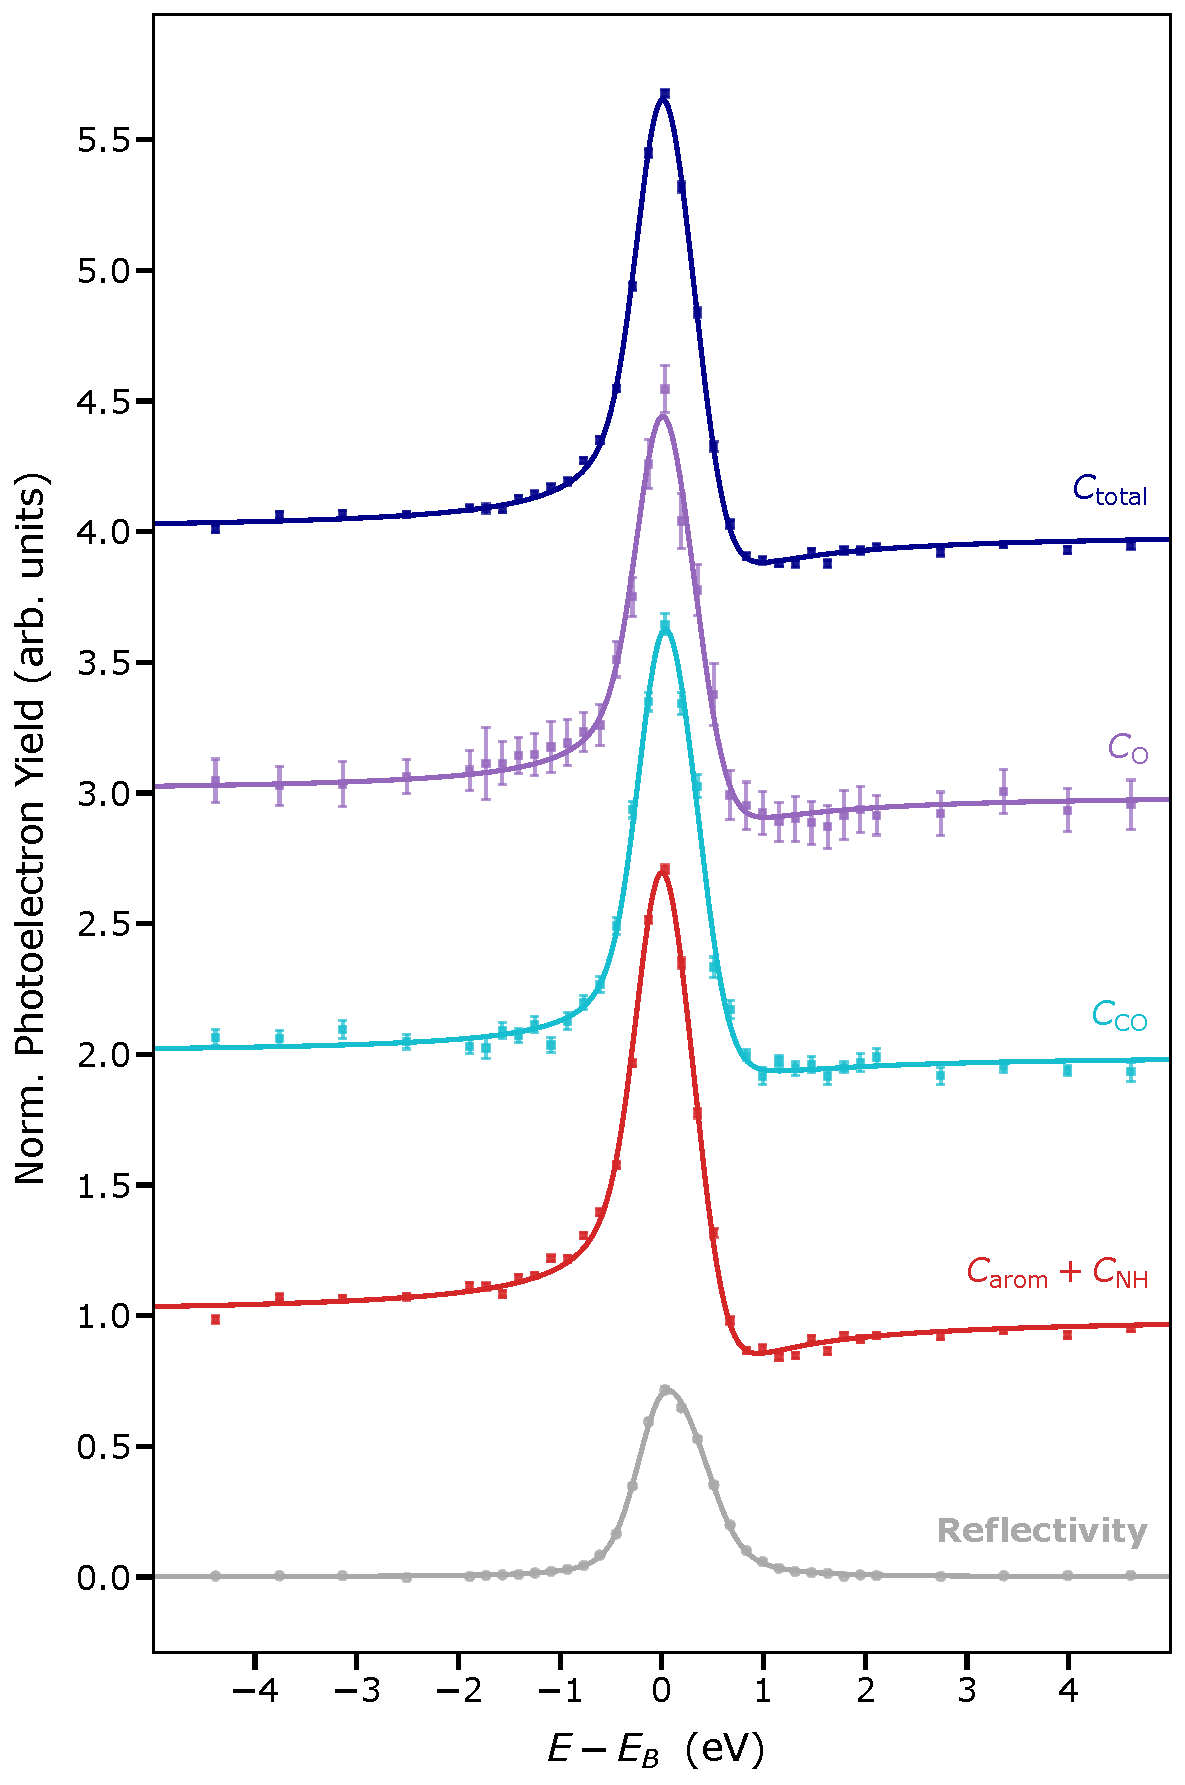
\includegraphics[width=0.8\textwidth]{images/NIXSW/NIXSW_C1s_Beta.pdf}
    \caption{C1s \ac{NIXSW} spectra of \ac{QA} on the Ag(100) surface in the $\beta$-phase. The sum of all components is shown at the top, followed by the individual components $\mathrm{C_{arom}}+\mathrm{C_{NH}}$, $\mathrm{C_{CO}}$ and $\mathrm{C_{O}}$ and the reflectivity at the bottom. For a better visibility, the different \ac{NIXSW} spectra are shifted vertically by 1. The fit parameter from \autoref{tab:XPS-C1s-fit-3peaks} were used for the individual \ac{XPS} spectra.}
    \label{fig:NIXSW-C1s-beta}
\end{figure}

The \ac{NIXSW} spectra in \autoref{fig:NIXSW-C1s-beta} show that the different C1s components exhibit only small changes in the \ac{NIXSW} spectra. This indicates that the different C atoms in the \ac{QA} molecule on the Ag(100) surface in the $\beta$-phase have similar coherent fractions and positions. The resulting fit parameters for the different C1s components are summarized in \autoref{tab:NIXSW-C1s-beta}.

\begin{table}[htbp]
	\centering
	\caption{Resulting coherent positions $p_\mathrm{c}$ and coherent fractions $p_\mathrm{c}$ for the different C1s components of \ac{QA} on the Ag(100) surface in the $\beta$-phase from \autoref{fig:NIXSW-C1s-beta}. The distance $z_{200}$ is calculated from the coherent position $p_\mathrm{c}$.}
	\begin{tabular}{@{}cccc@{}} \toprule
		 & $p_\mathrm{c}$ & $f_\mathrm{c}$ & $z_{200}$ (\si{\angstrom}) \\
		\midrule
		$\mathrm{C_{arom}}+\mathrm{C_{NH}}$ & $0.387 \pm 0.003$ & $0.758 \pm 0.017$ &  $2.834 \pm 0.006$ \\
		$\mathrm{C_{CO}}$ & $0.350 \pm 0.002$ & $0.660 \pm 0.025$ & $2.758 \pm 0.004$ \\ 
		$\mathrm{C_{O}}$ & $0.387 \pm 0.007$ & $0.564 \pm 0.026$ & $2.834 \pm 0.014$ \\
        $\mathrm{C_{total}}$ & $0.378 \pm 0.002$ & $0.712 \pm 0.012$ & $2.815 \pm 0.004$ \\
		\bottomrule
	\end{tabular}
	\label{tab:NIXSW-C1s-beta}
\end{table}

\autoref{tab:NIXSW-C1s-beta} shows that the different C1s components have coherent positions $p_\mathrm{c}$ between 0.350 and 0.387, which results in a coherent position $p_\mathrm{c}$ for the total C1s signal of 0.378. These values correspond to distances $z_{200}$ between 2.758~\si{\angstrom} and 2.834~\si{\angstrom}, with a distance of 2.815~\si{\angstrom} for the total C1s signal. It is important to note that the $\mathrm{C_{arom}}+\mathrm{C_{NH}}$ and $\mathrm{C_{O}}$ components have the same coherent position $p_\mathrm{c}$ of 0.387, but different coherent fractions $f_\mathrm{c}$ of 0.758 and 0.564, respectively.

In comparison to the $\alpha$-phase, the C atoms in the $\beta$-phase are located closer to the Ag(100) surface, with a difference in the distance $z_{200}$ of around 0.16~\si{\angstrom} (5~\%) for the total C1s signal. This means that the distance of the C atoms to the Ag(100) surface in the $\beta$-phase is lower than the sum of the van der Waals radii for C/Ag, which is 3.42~\si{\angstrom}\autocite{Bondi1964}, by 18~\%. Compared to the $\alpha$-phase, where the binding distance of the C atoms is only 13~\% closer to the surface than the van der Waals radii, the binding distance of the C atoms in the $\beta$-phase is significantly closer to the surface than in the $\alpha$-phase.

The binding distance of the C atoms in the $\beta$-phase is also significantly closer to the surface than the binding distance of the C atoms in \ac{PTCDA} on the Ag(100) surface, which is 2.84~\si{\angstrom}\autocite{Bauer2014}. As the merocyanine HB238 on the Ag(100) surface has a binding distance of 2.958~\si{\angstrom},\autocite{Kny2025} the binding distance of the C atoms of \ac{QA} to the Ag(100) surface in the $\beta$-phase is even more significantly smaller.

The coherent fractions $f_\mathrm{c}$ of the different C1s components in the $\beta$-phase are between 0.564 and 0.758, with a coherent fraction $f_\mathrm{c}$ of 0.712 for the total C1s signal. These values are significantly higher than the coherent fractions of the C1s components in the $\alpha$-phase, which are between 0.369 and 0.811, with a coherent fraction $f_\mathrm{c}$ of 0.523 for the total C1s signal.

In comparison to \ac{PTCDA} on the Ag(100) surface, which has a coherent fraction of 0.51 for the total C1s component,\autocite{Bauer2014} the C atoms in the \ac{QA} molecule on the Ag(100) surface in the $\beta$-phase have a significantly higher degree of order. Compared to the merocyanine HB238 on the Ag(100) surface, which has a coherent fraction of 0.242 for the C1s component,\autocite{Kny2025} the C atoms in the \ac{QA} molecule on the Ag(100) surface in the $\beta$-phase have a much higher degree of order.

\newpage
\subsection{N1s NIXSW spectra}

The N1s \ac{NIXSW} spectra of \ac{QA} on the Ag(100) surface in the $\beta$-phase are shown in \autoref{fig:NIXSW-N1s-beta}. At the bottom of the figure, the measured reflectivity curve of the (200) Bragg reflection is shown. The data points and the fitted curve of the N1s \ac{NIXSW} spectra are shown for the two \ac{XPS} components from \autoref{tab:XPS-N1s-fit} in different colors. At the top of the figure, the sum of all N1s components is shown. For a better visibility, the \ac{NIXSW} spectra are shifted vertically by 1.

\begin{figure}[htbp]
    \centering
    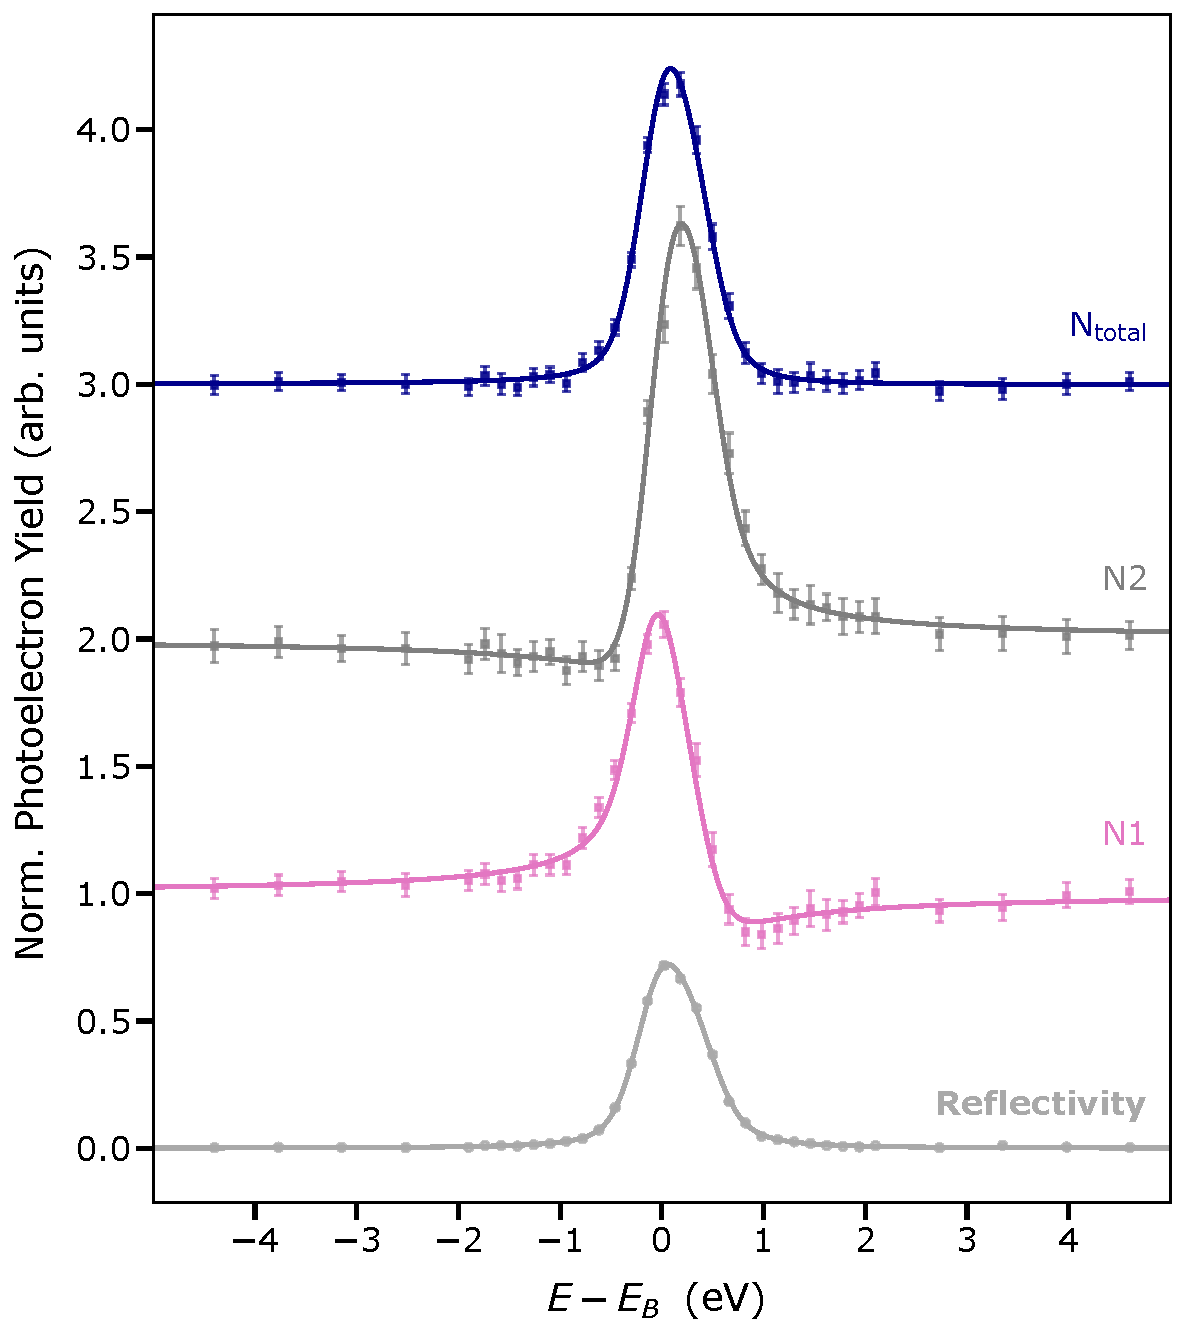
\includegraphics[width=0.8\textwidth]{images/NIXSW/NIXSW_N1s_Beta.pdf}
    \caption{N1s \ac{NIXSW} spectra of \ac{QA} on the Ag(100) surface in the $\beta$-phase. The sum of all components is shown at the top, followed by the individual components $\mathrm{N1}$ and $\mathrm{N2}$ and the reflectivity at the bottom. For a better visibility, the different \ac{NIXSW} spectra are shifted vertically by 1. The fit parameter from \autoref{tab:XPS-N1s-fit} were used for the individual \ac{XPS} spectra.}
    \label{fig:NIXSW-N1s-beta}
\end{figure}

\autoref{fig:NIXSW-N1s-beta} shows very different \ac{NIXSW} spectra for the two N1s components. The protonated N atom ($\mathrm{N1}$) has a coherent position $p_\mathrm{c}$ close to 0.5, which corresponds to a maximum followed by a minimum in the \ac{NIXSW} spectrum. In contrast, the deprotonated N atom ($\mathrm{N2}$) has a coherent position $p_\mathrm{c}$ close to 0.2, which corresponds to a minimum followed by a maximum in the \ac{NIXSW} spectrum. This opposite behavior indicates that the two N atoms in the \ac{QA} molecule on the Ag(100) surface in the $\beta$-phase are located at significantly different heights above the surface and explains the shape of the $\mathrm{N_{total}}$ peak with only one maximum.

The resulting fit parameters for the different N1s components are summarized in \autoref{tab:NIXSW-N1s-beta}.

\begin{table}[htbp]
	\centering
	\caption{Resulting coherent positions $p_\mathrm{c}$ and coherent fractions $p_\mathrm{c}$ for the different N1s components of \ac{QA} on the Ag(100) surface in the $\beta$-phase from \autoref{fig:NIXSW-N1s-beta}. The distance $z_{200}$ is calculated from the coherent position $p_\mathrm{c}$.}
	\begin{tabular}{@{}cccc@{}} \toprule
		 & $p_\mathrm{c}$ & $f_\mathrm{c}$ & $z_{200}$ (\si{\angstrom}) \\
		\midrule
		$\mathrm{N1}$ & $0.486 \pm 0.008$ & $0.374 \pm 0.021$ & $3.036 \pm 0.016$ \\
		$\mathrm{N2}$ & $0.184 \pm 0.004$ & $0.645 \pm 0.034$ & $2.419 \pm 0.008$ \\ 
        $\mathrm{N_{total}}$ & $0.289 \pm 0.005$ & $0.645 \pm 0.034$ & $2.633 \pm 0.010$ \\
		\bottomrule
	\end{tabular}
	\label{tab:NIXSW-N1s-beta}
\end{table}

The values in \autoref{tab:NIXSW-N1s-beta} show that the N1s components have coherent positions $p_\mathrm{c}$ of 0.486 and 0.184, which correspond to distances $z_{200}$ of 3.036~\si{\angstrom} and 2.419~\si{\angstrom}, respectively. This indicates a significant difference in height of 0.6~\si{\angstrom} between the two N atoms in the \ac{QA} molecule on the Ag(100) surface in the $\beta$-phase. This also means that the total N1s signal has a coherent position $p_\mathrm{c}$ of 0.289, which corresponds to a distance $z_{200}$ of 2.633~\si{\angstrom}, which is in between the distances of the two N atoms. However, as the two N atoms have very different coherent positions $p_\mathrm{c}$, the results of the total N1s signal are not very meaningful.

In comparison to the $\alpha$-phase, where the N atoms have a coherent position $p_\mathrm{c}$ of 0.499, which corresponds to a distance $z_{200}$ of 3.062~\si{\angstrom}, the N1 component in the $\beta$-phase has a similar coherent position $p_\mathrm{c}$ and thus a similar distance to the surface as the N atoms in the $\alpha$-phase. As already stated above, the deprotonated N2 component has a significantly distance $z_{200}$ of 2.419~\si{\angstrom}. This means that the deprotonated N atom in the $\beta$-phase is located significantly closer to the Ag(100) surface than the not deprotonated N atoms in the $\alpha$ and $\beta$-phase, with a difference in the distance $z_{200}$ of around 0.64~\si{\angstrom} (21~\%).

Again, this the distance of the deprotonated N atom to the Ag(100) surface in the $\beta$-phase is significantly smaller than the sum of the van der Waals radii for N/Ag, which is 3.30~\si{\angstrom}\autocite{Bondi1964}, by 27~\%. This is a significant difference compared to the N atoms in the $\alpha$-phase, which are only 7~\% closer to the surface than the van der Waals radii.

The coherent fractions $f_\mathrm{c}$ are 0.374 for the N1 component and 0.645 for the deprotonated N2 component, indicating very different degrees of order for the two N atoms. Compared to the $\alpha$-phase, where the N atoms have a coherent fraction $f_\mathrm{c}$ of 0.288, the N1 component in the $\beta$-phase has a higher degree of order, while the deprotonated N2 component has a significantly higher degree of order than the N atoms in the $\alpha$-phase.

\newpage
\subsection{O1s NIXSW spectra}

The O1s \ac{NIXSW} spectra of \ac{QA} on the Ag(100) surface in the $\beta$-phase are shown in \autoref{fig:NIXSW-O1s-beta}. At the bottom of the figure, the measured reflectivity curve of the (200) Bragg reflection is shown. The data points and the fitted curve of the O1s \ac{NIXSW} spectra are shown for the two \ac{XPS} components from \autoref{tab:XPS-O1s-fit} in different colors. At the top of the figure, the sum of all O1s components is shown. For a better visibility, the \ac{NIXSW} spectra are shifted vertically by 1.

\begin{figure}[htbp]
    \centering
    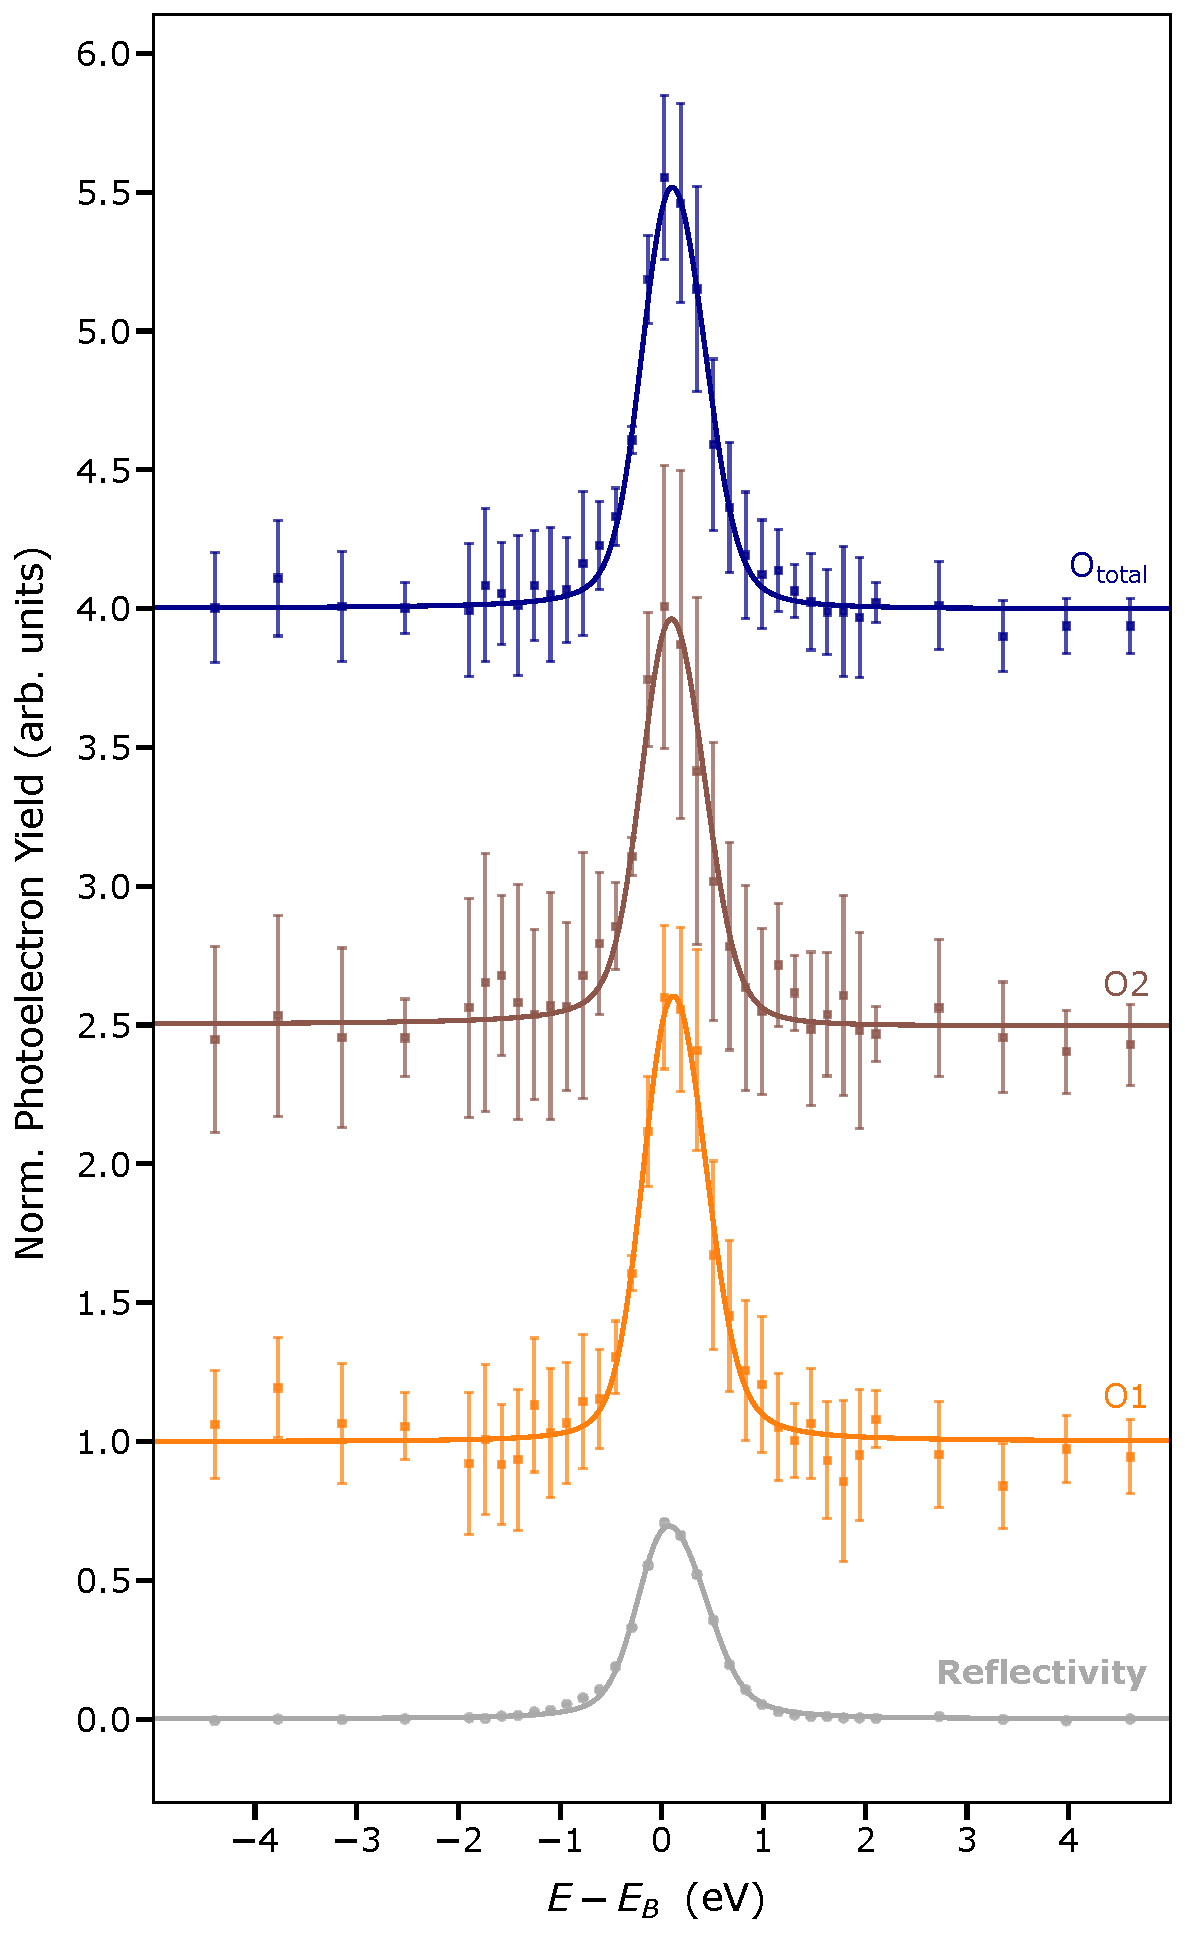
\includegraphics[width=0.8\textwidth]{images/NIXSW/NIXSW_O1s_Beta.pdf}
    \caption{O1s \ac{NIXSW} spectra of \ac{QA} on the Ag(100) surface in the $\beta$-phase. The sum of all components is shown at the top, followed by the individual components $\mathrm{O1}$ and $\mathrm{O2}$ and the reflectivity at the bottom. For a better visibility, the different \ac{NIXSW} spectra are shifted vertically by 1. The fit parameter from \autoref{tab:XPS-O1s-fit} were used for the individual \ac{XPS} spectra.}
    \label{fig:NIXSW-O1s-beta}
\end{figure}

As seen in \autoref{fig:NIXSW-O1s-beta}, the different O1s components exhibit almost identical \ac{NIXSW} spectra. This indicates that the different O atoms in the \ac{QA} molecule on the Ag(100) surface in the $\beta$-phase have very similar coherent fractions and positions.

The resulting coherent positions $p_\mathrm{c}$ and coherent fractions $f_\mathrm{c}$ for the different O1s components of \ac{QA} on the Ag(100) surface in the $\beta$-phase from \autoref{fig:NIXSW-O1s-beta} are summarized in \autoref{tab:NIXSW-O1s-beta}. The distance $z_{200}$ is calculated from the coherent position $p_\mathrm{c}$.

\begin{table}[htbp]
	\centering
	\caption{Resulting coherent positions $p_\mathrm{c}$ and coherent fractions $p_\mathrm{c}$ for the different O1s components of \ac{QA} on the Ag(100) surface in the $\beta$-phase from \autoref{fig:NIXSW-O1s-beta}. The distance $z_{200}$ is calculated from the coherent position $p_\mathrm{c}$.}
	\begin{tabular}{@{}cccc@{}} \toprule
		 & $p_\mathrm{c}$ & $f_\mathrm{c}$ & $z_{200}$ (\si{\angstrom}) \\
		\midrule
		$\mathrm{O1}$ & $0.272 \pm 0.007$ & $0.658 \pm 0.056$ & $2.599 \pm 0.014$ \\
		$\mathrm{O2}$ & $0.291 \pm 0.011$ & $0.559 \pm 0.072$ & $2.638 \pm 0.022$ \\ 
        $\mathrm{O_{total}}$ & $0.282 \pm 0.006$ & $0.598 \pm 0.042$ & $2.619 \pm 0.012$ \\
		\bottomrule
	\end{tabular}
	\label{tab:NIXSW-O1s-beta}
\end{table}

\autoref{tab:NIXSW-O1s-beta} shows that the O1s components have coherent positions $p_\mathrm{c}$ of 0.272 and 0.291, which correspond to distances $z_{200}$ of 2.599~\si{\angstrom} and 2.638~\si{\angstrom}, respectively. Taking the errors of these two values into account, the two O atoms in the \ac{QA} molecule on the Ag(100) surface in the $\beta$-phase are located at similar heights above the surface. The total O1s signal has a coherent position $p_\mathrm{c}$ of 0.282, which corresponds to a distance $z_{200}$ of 2.619~\si{\angstrom}, which is in between the distances of the two O atoms.

In comparison to the $\alpha$-phase, where the O atoms have a distance $z_{200}$ of 2.721~\si{\angstrom}, the O1 component in the $\beta$-phase has a lower distance to the Ag(100) surface than the O atoms in the $\alpha$-phase, with a difference in the distance $z_{200}$ of around 0.12~\si{\angstrom} (4~\%). This difference in the distance $z_{200}$ is similar to the difference of the C atoms between the $\alpha$-phase and the $\beta$-phase, which is around 0.16~\si{\angstrom} (5~\%). This shows that both the C atoms and the O atoms are located closer to the Ag(100) surface in the $\beta$-phase compared to the $\alpha$-phase.

The distance of the O atoms to the Ag(100) surface in the $\beta$-phase is also significantly smaller than the sum of the van der Waals radii for O/Ag, which is 3.24~\si{\angstrom}\autocite{Bondi1964}, by around 20~\%. 

For the N atoms, two different heights of the two N atoms above the surface were observed, whereas the O atoms are located at similar heights above the surface. This is a significant difference between the N and O atoms, which form hydrogen bonds between the neighboring molecules with the N1/O1 component and do not form hydrogen bonds between the N2/O2 component due to the deprotonation of the N2 component.

In comparison to \ac{PTCDA} on the Ag(100) surface, which has a distance of 2.53~\si{\angstrom} for the O atoms,\autocite{Bauer2014} the O atoms in the \ac{QA} molecule on the Ag(100) surface in the $\beta$-phase are located farther away from the surface by 0.09~\si{\angstrom}. 

The coherent fractions $f_\mathrm{c}$ of the O1 and O2 components are 0.658 and 0.559, respectively. The total O1s signal has a coherent fraction $f_\mathrm{c}$ of 0.598. This shows that the O atoms have similar degrees of order, which is in agreement with the similar heights of the O atoms.

Compared to the $\alpha$-phase, where the O atoms have a coherent fraction $f_\mathrm{c}$ of 0.546, the O1 and O2 components in the $\beta$-phase have a higher degree of order. Furthermore, the O atoms in the \ac{QA} molecule on the Ag(100) surface in the $\beta$-phase have also a higher degree of order than the O atoms in \ac{PTCDA} on the Ag(100) surface, which have a coherent fraction of 0.51.\autocite{Bauer2014}


\newpage
\subsection{Argand representation for the \texorpdfstring{$\beta$}{beta}-phase}

To summarize the resulting coherent positions and fractions for the different core levels of \ac{QA} on the Ag(100) surface in the $\beta$-phase, an Argand representation is shown in \autoref{fig:Argand-beta}. Here, the coherent position $p_\mathrm{c}$ is represented as the angle and the coherent fraction $f_\mathrm{c}$ as the distance from the origin.

\begin{figure}[htbp]
	\centering
	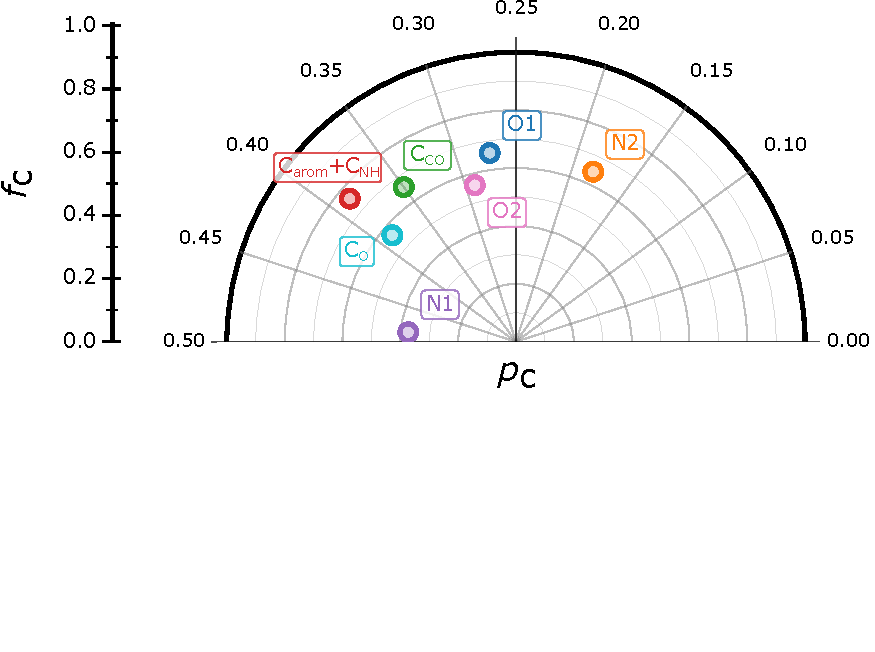
\includegraphics[width=\textwidth]{images/NIXSW/Argand_Beta_2.pdf}
	\caption{Argand representation for \ac{QA} on the Ag(100) surface in the $\beta$-phase for the C1s, N1s, and O1s core levels.}
	\label{fig:Argand-beta}
\end{figure}

\autoref{fig:Argand-beta} shows that the different core levels of \ac{QA} on the Ag(100) surface in the $\beta$-phase have more varying coherent fractions $f_\mathrm{c}$ and coherent positions $p_\mathrm{c}$ compared to the $\alpha$-phase, indicating that the different atoms in the \ac{QA} molecule are located at more diverse heights above the Ag(100) surface. 

All C1s components have similar coherent positions $p_\mathrm{c}$ and thus similar heights above the surface. However, there are slight differences between the $\mathrm{C_{arom}}+\mathrm{C_{NH}}$, $\mathrm{C_{CO}}$ and $\mathrm{C_{O}}$ components. The $\mathrm{C_{CO}}$ component has the lowest coherent position $p_\mathrm{c}$ of 0.350, but the $\mathrm{C_{arom}}+\mathrm{C_{NH}}$ and $\mathrm{C_{O}}$ components have the same coherent position $p_\mathrm{c}$ of 0.387, which is higher than the coherent position $p_\mathrm{c}$ of the $\mathrm{C_{CO}}$ component. This shows that the C atoms in the \ac{QA} molecule are not in a perfect plane but slightly distorted.

The C1s component also have different coherent fractions $f_\mathrm{c}$, with the $\mathrm{C_{arom}}+\mathrm{C_{NH}}$ component having the highest coherent fraction $f_\mathrm{c}$ of 0.758, followed by the $\mathrm{C_{CO}}$ component with a coherent fraction $f_\mathrm{c}$ of 0.660 and the $\mathrm{C_{O}}$ component with a coherent fraction $f_\mathrm{c}$ of 0.564. This shows that the $\mathrm{C_{arom}}+\mathrm{C_{NH}}$ component has the highest degree of order, while the $\mathrm{C_{O}}$ component has the lowest degree of order. However, the differences in the coherent fractions $f_\mathrm{c}$ are also affected by the different signal-to-noise ratios of the different components, which can lead to higher errors for the components with lower signal-to-noise ratios and thus to a less reliable determination of the coherent fractions $f_\mathrm{c}$.

The N1 and N2 components have very different coherent positions $p_\mathrm{c}$, with the N1 component having a coherent position $p_\mathrm{c}$ of 0.486 and the N2 component having a coherent position $p_\mathrm{c}$ of 0.184. It is important to note that the N2 component is the deprotonated N atom, which does not form a hydrogen bond to the neighboring molecule, while the N1 component is the protonated N atom, which forms a hydrogen bond to the neighboring molecule. This shows that the deprotonation of the N2 component leads to a significantly different adsorption behavior of this N atom compared to the protonated N1 component.

The deprotonated N atom is located significantly closer to the Ag(100) surface than the protonated N atom. This could be explained by the fact that the deprotonated N atom has a high electron density due to the electron lone pair, which can lead to a stronger interaction between the deprotonated N atom and the Ag(100) surface due to a donation of electron density from the deprotonated N atom to the Ag(100) surface. In addition, this shows that the adsorption height of the deprotonated N atom is mostly influenced by the interaction with the Ag(100) surface.

In contrast, the protonated N atom has a similar distance to the surface as the N atoms in the $\alpha$-phase. This shows that the interaction between the protonated N atom and the Ag(100) surface is not significantly altered by the phase transition from the $\alpha$-phase to the $\beta$-phase. Furthermore, it also shows that the adsorption height of the protonated N atom is mostly influenced by the hydrogen bond to the neighboring molecule.

The coherent fractions $f_\mathrm{c}$ of the N1 and N2 components are also very different, with the N1 component having a coherent fraction $f_\mathrm{c}$ of 0.374 and the N2 component having a coherent fraction $f_\mathrm{c}$ of 0.645. This shows that the deprotonated N2 component has a significantly higher degree of order than the protonated N1 component, which could be explained by its stronger interaction with the Ag(100) surface, which leads to a more well-defined adsorption height for the deprotonated N2 component compared to the protonated N1 component.

The protonated N1 component has a higher coherent fraction $f_\mathrm{c}$  by 0.9 as the N atoms in the $\alpha$-phase, which shows that the degree of order of the protonated N1 component is altered by the phase transition from the $\alpha$-phase to the $\beta$-phase, but not as much as for the deprotonated N2 component. This indicates that the adsorption height of the protonated N1 component is mostly influenced by the hydrogen bond to the neighboring molecule.

Last, the O1 and O2 components have similar coherent positions $p_\mathrm{c}$ and thus similar heights above the surface, which is closer to the surface than in the $\alpha$-phase. This shows that the O atom with and the O atom without a hydrogen bond to the neighboring molecule have similar adsorption heights. Consequently, the interaction between the O atoms and the Ag(100) surface is more important than the interaction by intermolecular hydrogen bonds for the adsorption height. 

This behaviour is the opposite to the N atoms, where the adsorption height strongly depends on the presence of a hydrogen bond to the neighboring molecule. This can be explained by the fact that the electron density of the O atoms with or without a hydrogen bond does not change as significant as the electron density of the N atoms between the protonated and deprotonated state.

The coherent fractions $f_\mathrm{c}$ of the O1 and O2 components are different by 0.099, with the O1 component having a coherent fraction $f_\mathrm{c}$ of 0.658 and the O2 component having a coherent fraction $f_\mathrm{c}$ of 0.559. This shows that the O1 component, which forms a hydrogen bond to the neighboring molecule, has a higher degree of order than the O2 component, which does not form a hydrogen bond to the neighboring molecule. This indicates that the hydrogen bond to the neighboring molecule has a small influence on the degree of order of the O atoms in the \ac{QA} molecule, even though the adsorption height of the O atoms is mostly influenced by the interaction with the Ag(100) surface.



\cleardoublepage